\chapter{基于web可视化工具概述}
\chaptermark{基于web可视化工具概述}
	\section{GBrowse}
		\subsection{概述}
		GBrowse是基因组浏览器(GenomeBrowse)的缩写。它是一种基于WE
		\subsection{可视化方式}
		GBrowse用 track的方式进行可视化相关基因组信息,通过对track进行缩放。通过合理地配置及编码可以实现基因组基因的可视化。
	
		\subsection{可视化内容}
		GBrowse可视化内容由可视化图谱进行具体显示,可视化图谱可以分为三个部分:overview(概述),region(区域),details(细节)。
		\begin{itemize}
		
		\end{itemize}

		\begin{figure}
			\centering
			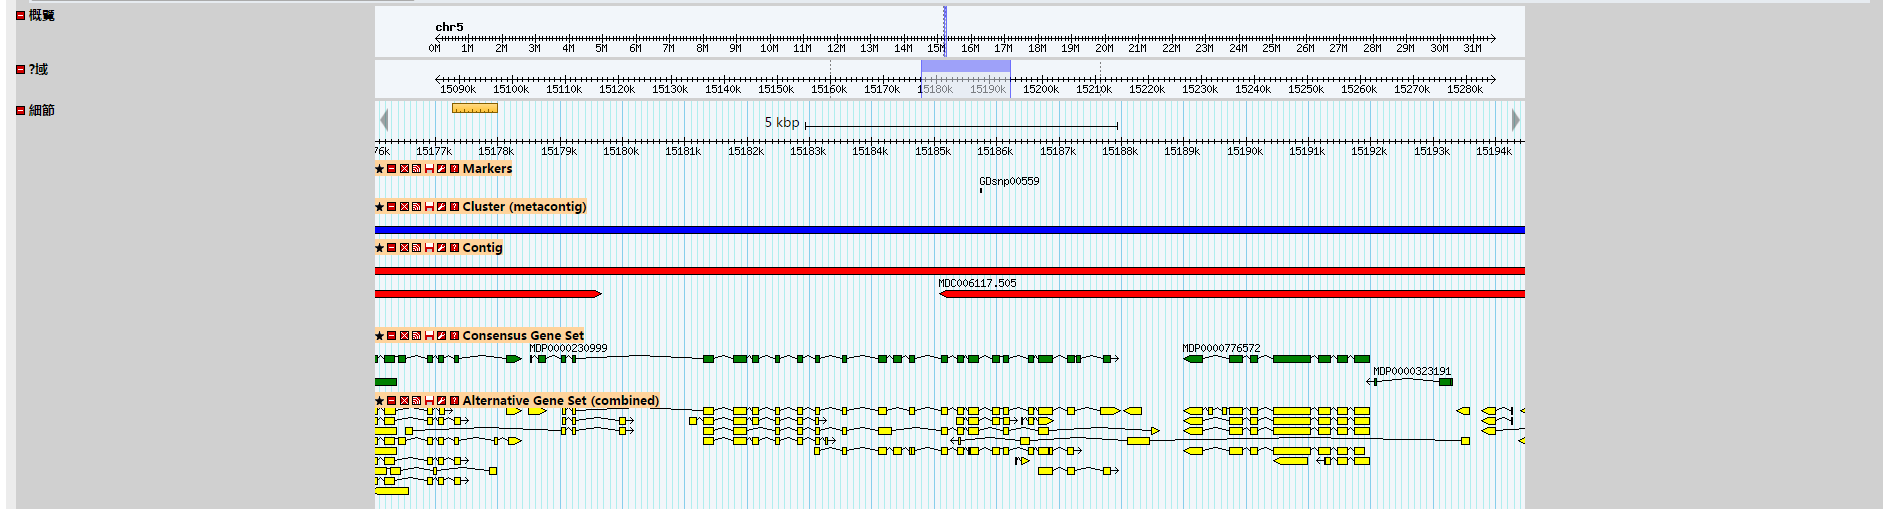
\includegraphics[width = .9\textwidth]{2-1.png}
			\caption{GBrowse页面内容展示图}
		\end{figure}	
		\subsection{系统架构}
		GBrowse是一个Web应用程序,可分为Web服务器端和Web浏览器客户,它将数子到SNP单倍型区段之间的连锁不平衡的高度特异性表示。
		\begin{figure}[!ht]
			\centering
			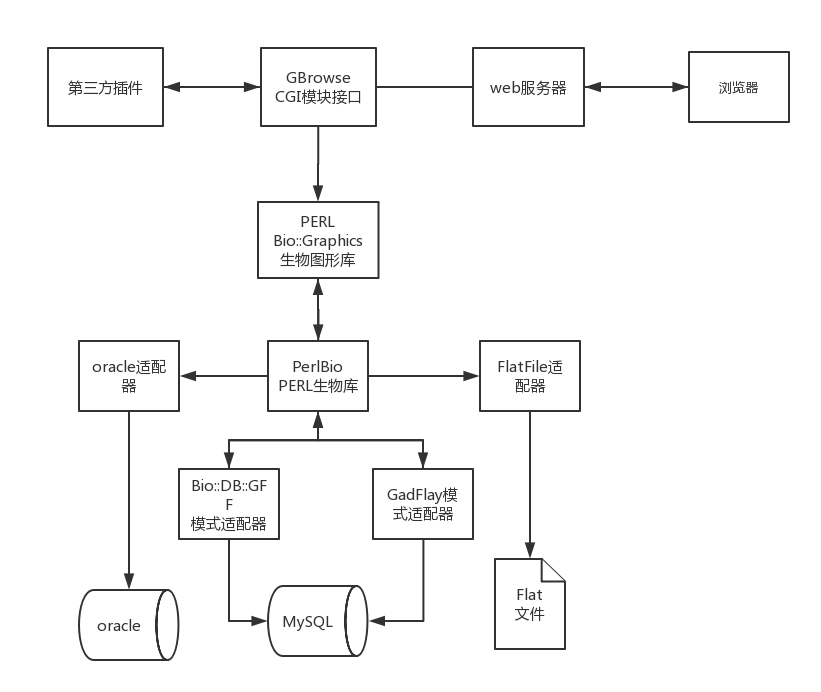
\includegraphics[width = .6\textwidth]{2-2.png}
			\caption{GBrowse系统结构}
		\end{figure}
		\subsection{运行机理}
产生可视化效果。如图2-3GBrowse的CGI模块请求处理流程。
			\begin{figure}[!ht]
				\centering
				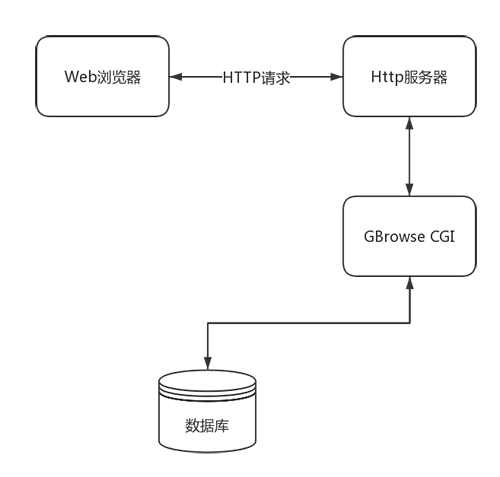
\includegraphics[width = .5\textwidth]{2-3.png}
				\caption{GBrowse模块请求处理}
			\end{figure}
		\subsection{优缺点}
		优点:GBrowse支持大部分基因组数据集格式,对于浏览器的兼容性良好,可以友好的显示在web端,并且拥有良好的跨平台性和兼容性;GBrows
		%JBrowse
	\section{JBrowse}
		\subsection{概述}
	台应用开发框架下逐步推出Windows等操作系统下的应用软件,方便用户可视化数据。
		\subsection{可视化方式}
		JBrowse用 track 的方式进行可视化,提供平滑的动态移动和缩放功能,也有导航和通道的选择。JBrowse可以展示多种 track 视图,除基本视图外,还可以显示非翻译区、外显子、内含子结构等。
		
		\subsection{可视化内容}
		JBrowse可以展示基因组整体视图,也可以细化展示基因跨度、tRNA、转座子、寡核苷酸、蛋白质结合位点、增强子、基因调控区域、非编码RNA、点突变、序列变异信息等其它基因信息。用户可以自己上传需要可视化的内容的相关基因数据,支持GFF、GFF3、WIG、BED、FASTA、Wiggle、BigWig、BAM 等多种格式的数据文件。如图2-5所示
		\begin{figure}[!ht]
			\centering
			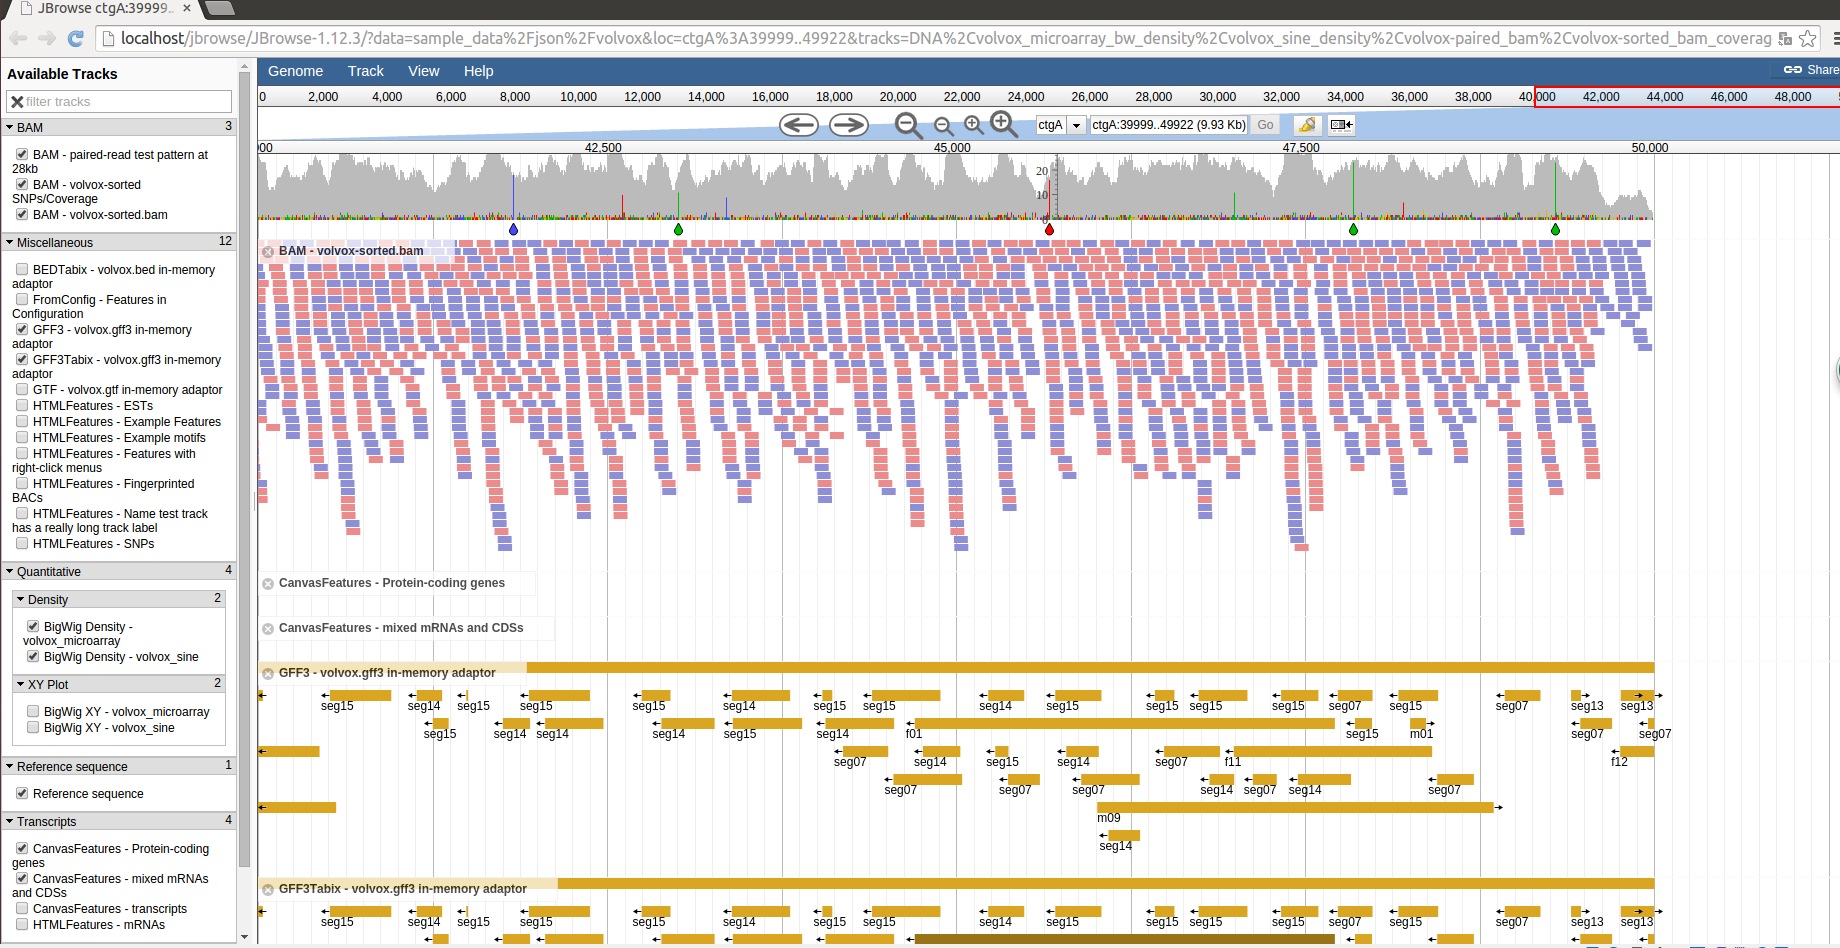
\includegraphics[width = .6\textwidth]{2-4.png}
			\caption{JBrowse可视化内容}
		\end{figure}
		\subsection{系统架构}
配器由Perl编写实现,有易扩展的特性;JBrowse对多种数据适配器支持,比如Bio::DB::SeqFeature::Store,数据适配器的多样使JBrowse支持多种数据类TP请求发送过来的tile索引文件并检索和组织图片进行显示,并且可以将渲染的图片扩展到任意维度。JBrowse通过使用Html及Canvas来显示图形内容。
		\begin{figure}[!ht]
			\centering
			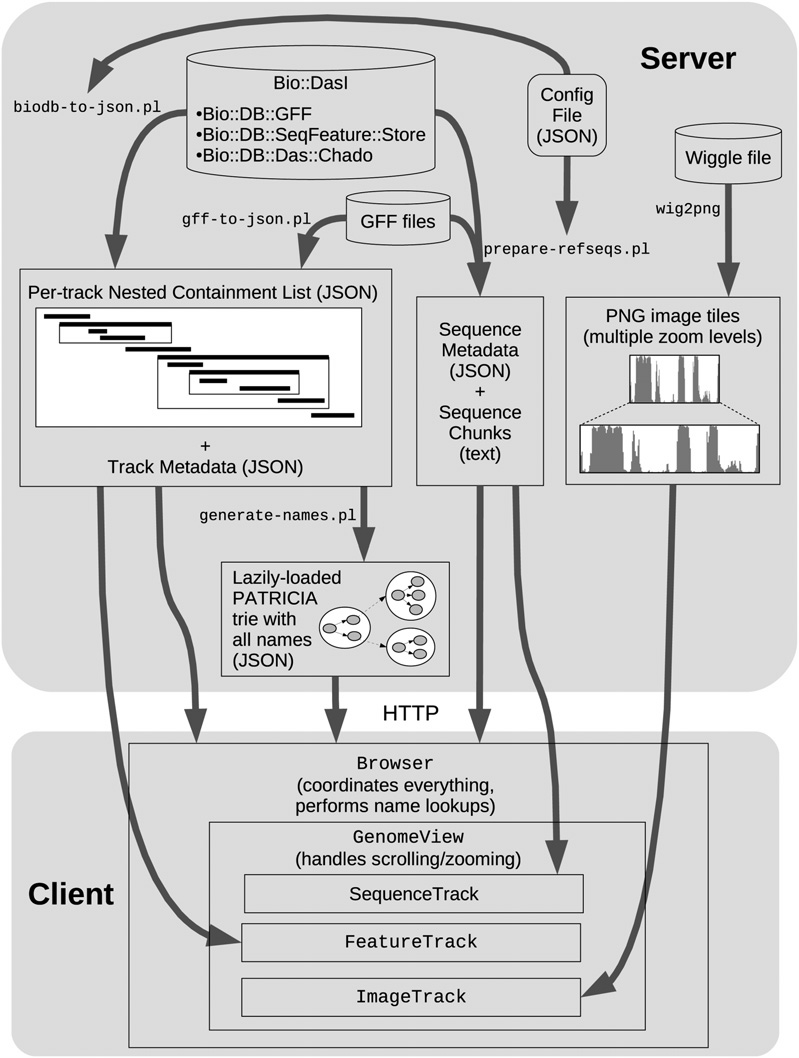
\includegraphics[width = .4\textwidth]{2-5.png}
			\caption{JBrowse系统架构}
		\end{figure}
		\subsection{运行机理}
		JBrowse的工作流分为服务端工作流和前端工作流。当用户通过浏览器对目标网址进行访问时服务端将预处理后的数据进行以Json的形式进行传送到前端,前端通过Javascript引擎进行加载处理,并渲染生成基因数据图像。\\
		\indent 服务端将对于后端工作流大致可以概括为基本调用,汇编,注释,对齐和比较注释,并生成了JBrowse文件。服务端将序列文件进行注释,对比注释,phastCons等操作对数据进一步进行数据整理和压缩,通过HTTP请求进行数具传输。
		\begin{figure}[!ht]
			\centering
			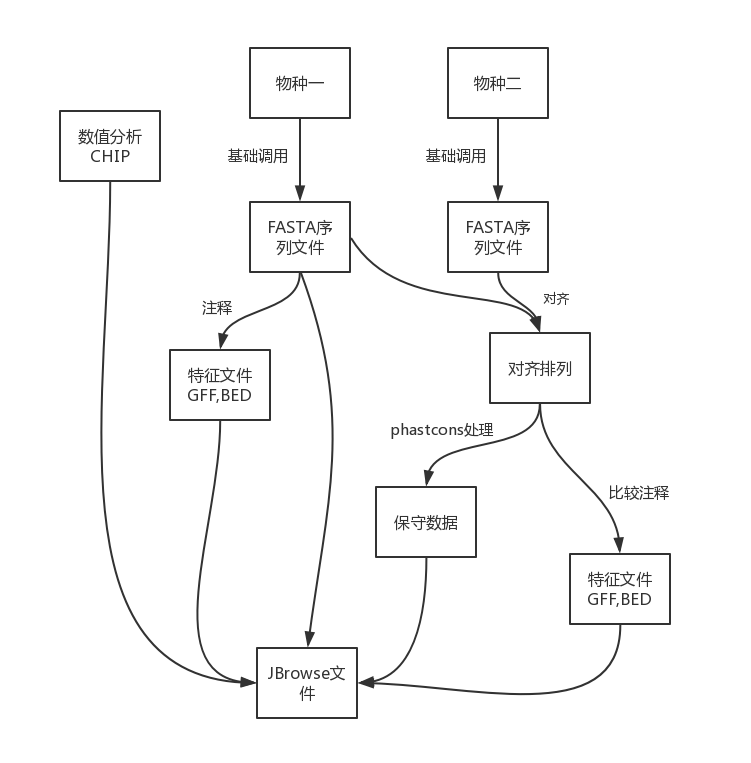
\includegraphics[width = .4\textwidth]{2-6.png}
			\caption{JBrowse工作流图}
		\end{figure}
		\subsection{优缺点}
		优点:流浏览器对 HTML5 中新标签的支持不完善,造成用户体验不佳等问题。
	\section{UCSC Genome Browser}		
			\subsection{概述}	
			UCSC Genome Browser是由University of California Santa Cruz 育或科研目的加上他们自己的注释信息。
			\subsection{可视化方式}		
			。 
			\begin{figure}[!ht]
				\centering
				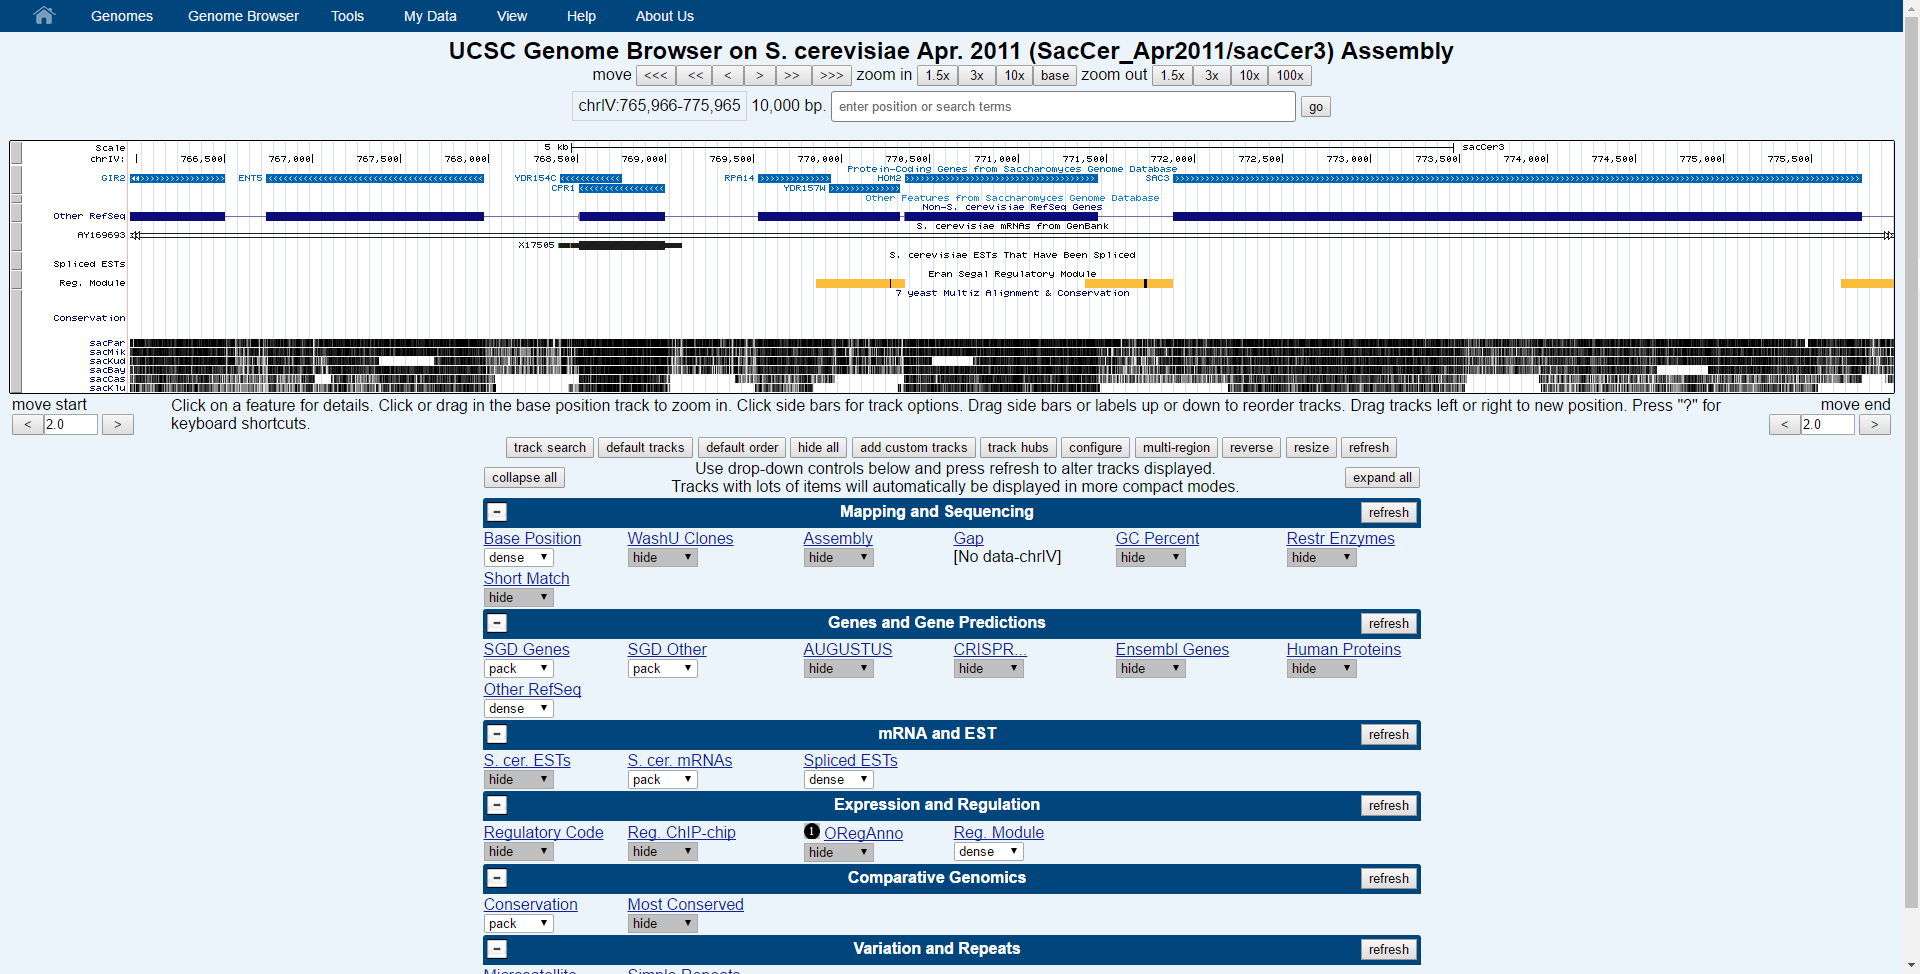
\includegraphics[width = .4\textwidth]{2-7.png}
				\caption{UCSC Genome Browser系统界面}
			\end{figure}
			\subsection{可视化内容}		
			
			\subsection{系统架构}		
			UCSC Genome Browser 的开发,起源于一小段应用于 C. elegans 基因预测拼接图谱的 C 语言脚本,后期通过不断扩充,才变成现在这样强大的一个分析工具。 现在 UCSC 的主要开发语言是Java/Python,后台数据库依赖于 mysql,而且提供mysql 的公共接口,只要用户本地电脑装有 mysql客户端,就可以通过 UCSC 提供的接口访问网站后台的数据库;对于前台要求,UCSC 可以较好地兼容 IE、Chrome、Firefox 等主流网络浏览器。UCSC 是完全开源的,用户可以下载到完整源码。
			\subsection{优缺点}
			优点:	UCSC Genome Browser 是一个非常综合的基因组浏览器,包含物种数比较多,可视化内容也比较齐全。\\
			\indent 缺点:从 web 